% !TeX root = ../main.tex
\section{Домашняя подготовка}
% Создать шаблон отчета для результатов домашней подготовки и лабораторного задания[cite: 4]

\subsection{Схемы формирования дальномерного кода}
% Изучить разделы ИКД ГЛОНАСС L1 СТ и GPS L1 C/A, посвященные схемам формирования дальномерного кода. Привести схемы блоков формирования дальномерного кода в отчете.[cite: 4]

\subsubsection{Схема формирования ПСП ГЛОНАСС L1 СТ}
% Место для TikZ-схемы 9-разрядного регистра сдвига с полиномом G(x) = 1 + x^5 + x^9
\begin{figure}[H]
    \centering
    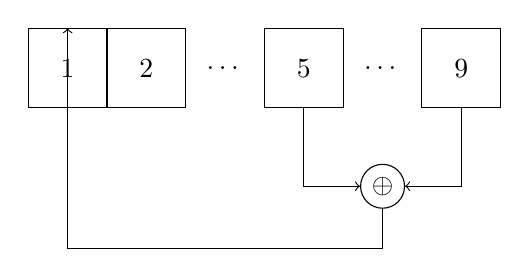
\begin{tikzpicture}[box/.style={draw, minimum width=1cm, minimum height=1cm, align=center}]
        % Пример базовой разметки для блоков, заполнить при необходимости
        \node[box] (reg1) at (0,0) {1};
        \node[box] (reg2) at (1,0) {2};
        \node at (2,0) {\dots};
        \node[box] (reg5) at (3,0) {5};
        \node at (4,0) {\dots};
        \node[box] (reg9) at (5,0) {9};
        
        % Связи и XOR
        \node[draw, circle, inner sep=2pt] (xor) at (4,-1.5) {$\oplus$};
        \draw[->] (reg5.south) |- (xor.west);
        \draw[->] (reg9.south) |- (xor.east);
        \draw[->] (xor.south) -- ++(0,-0.5) -| (reg1.north);
    \end{tikzpicture}
    \caption{Структурная схема генератора дальномерного кода ГЛОНАСС L1 СТ}
\end{figure}

\subsubsection{Схема формирования ПСП GPS L1 C/A}
% Место для TikZ-схемы генератора кодов Голда (два 10-разрядных регистра)
\begin{figure}[H]
    \centering
    % Добавить схему G1 и G2
    \caption{Структурная схема генератора дальномерного кода GPS L1 C/A}
\end{figure}

\subsection{Статистические эквиваленты выходных отсчетов коррелятора}
% Привести выражения для статистических эквивалентов выходных отсчетов коррелятора.[cite: 4]

Математические ожидания квадратурных сумм после накопления (статистические эквиваленты) определяются следующими выражениями:

\begin{equation}
    M[I_k] = \frac{A}{2} N R(\Delta \tau_k) \frac{\sin(\pi \Delta f_k T)}{\pi \Delta f_k T} \cos(\Delta \varphi_k)
\end{equation}

\begin{equation}
    M[Q_k] = \frac{A}{2} N R(\Delta \tau_k) \frac{\sin(\pi \Delta f_k T)}{\pi \Delta f_k T} \sin(\Delta \varphi_k)
\end{equation}

где:
\begin{itemize}
    \item $A$ — амплитуда сигнала;
    \item $N$ — количество отсчетов на интервале накопления;
    \item $T$ — интервал накопления;
    \item $R(\Delta \tau_k)$ — значение автокорреляционной функции дальномерного кода при ошибке по задержке $\Delta \tau_k$;
    \item $\Delta f_k$ — ошибка по частоте;
    \item $\Delta \varphi_k$ — ошибка по фазе.
\end{itemize}

\newpage
\section{Результаты лабораторного исследования}

\subsection{Идеальные условия приема (Бесконечная полоса, без шума)}
% Отключить шум приемного устройства. В качестве значения полосы фронтенда выбрать «Бесконечность». Квантование принимаемой реализации и опорного сигнала отключить. Расстройку опорного сигнала по частоте установить нулевой. На основании ИКД установить параметры схемы формирования ДК. Перенести схему в отчет. Занести в отчет вычисленные корреляционные функции. Определить промежуточную частоту сигнала, полосу сигнала.[cite: 4]

\textbf{Параметры схемы формирования ДК (из интерфейса программы):}
\begin{itemize}
    \item Обратные связи регистра: % Указать задействованные отводы
    \item Начальное состояние: % Указать вектор начального состояния
\end{itemize}

\begin{figure}[H]
    \centering
    % \includegraphics[width=0.8\textwidth]{images/scheme_infinite_bw.png}
    \caption{Схема формирования ДК в интерфейсе модели}
\end{figure}

\begin{figure}[H]
    \centering
    % \includegraphics[width=0.8\textwidth]{images/corr_infinite_bw.png}
    \caption{Вычисленные корреляционные функции (Полоса: Бесконечность)}
\end{figure}

\textbf{Определенные параметры:}
\begin{itemize}
    \item Промежуточная частота сигнала $f_{if} = $ % Вписать значение
    \item Полоса сигнала $\Delta f_c = $ % Вписать значение
\end{itemize}

\subsection{Влияние ограничения полосы пропускания фронтенда}
% Установить полосу фронтенда равной 6 МГц, 1 МГц. Перенести корреляционные функции в отчет. Оценить групповое время запаздывания.[cite: 4]

\begin{figure}[H]
    \centering
    % \includegraphics[width=0.48\textwidth]{images/corr_6mhz.png}
    % \includegraphics[width=0.48\textwidth]{images/corr_1mhz.png}
    \caption{Корреляционные функции при полосе фронтенда 6 МГц (слева) и 1 МГц (справа)}
\end{figure}

\textbf{Оценка группового времени запаздывания:}
\begin{itemize}
    \item Для полосы 6 МГц: $t_{гвз} \approx $ % Вписать значение
    \item Для полосы 1 МГц: $t_{гвз} \approx $ % Вписать значение
\end{itemize}

\subsection{Воздействие собственного шума приемника}
% В качестве значения полосы фронтенда выбрать «6 МГц». Перенести в отчет наглядный отрезок сигнала. Включить шум. Сравнить квадрат СКО шума (считая размах за 3 СКО) и мощность сигнала. Определить отношение мощности сигнала к односторонней спектральной плотности шума. Перенести в отчет отрезок реализации сигнала в смеси с шумом, корреляционные функции.[cite: 4, 5]

\begin{figure}[H]
    \centering
    % \includegraphics[width=0.8\textwidth]{images/signal_6mhz_nonoise.png}
    \caption{Отрезок сигнала (полоса 6 МГц, без шума)}
\end{figure}

\begin{figure}[H]
    \centering
    % \includegraphics[width=0.8\textwidth]{images/signal_6mhz_noise.png}
    \caption{Отрезок реализации сигнала в смеси с шумом}
\end{figure}

\textbf{Расчет энергетических параметров:}
\begin{itemize}
    \item Квадрат СКО шума $\sigma_n^2 \approx $ % Расчет
    \item Мощность сигнала $P_c \approx $ % Расчет
    \item Отношение $P_c / N_0 = $ % Расчет в дБГц
\end{itemize}

\begin{figure}[H]
    \centering
    % \includegraphics[width=0.8\textwidth]{images/corr_6mhz_noise.png}
    \caption{Корреляционные функции при наличии шума (полоса 6 МГц)}
\end{figure}

% Наблюдать за изменением шумовой составляющей корреляционных функций при изменении полосы фронтенда. Исследовать зависимость мощности шумовой составляющей корреляционных компонент от полосы фронтенда, сделать соответствующие записи в отчете.[cite: 5]
\textbf{Зависимость мощности шумовой составляющей от полосы фронтенда:}\\
% Описание наблюдений за изменением шумовой дорожки на графиках I и Q при переключении полосы (Бесконечность -> 6 МГц -> 1 МГц)

\subsection{Влияние ошибки по частоте}
% Выключить шум. Варьируя ошибку по частоте с шагом 200 Гц в диапазоне от -2 до +2 кГц, составить таблицу зависимости от ошибки по частоте компонент Ip, Qp при нулевой ошибке по задержке. Сравнить результат со статистическим эквивалентом.[cite: 5]

\begin{table}[H]
    \centering
    \caption{Зависимость компонент $I_p, Q_p$ от ошибки по частоте ($\Delta \tau = 0$)}
    \begin{tabular}{@{}ccccc@{}}
        \toprule
        $\Delta f$, Гц & $I_p$ (модель) & $Q_p$ (модель) & $M[I_p]$ (стат. экв.) & $M[Q_p]$ (стат. экв.) \\ \midrule
        -2000 & & & & \\
        -1800 & & & & \\
        \dots & & & & \\
        0 & & & & \\
        \dots & & & & \\
        +2000 & & & & \\ \bottomrule
    \end{tabular}
\end{table}

\textbf{Анализ результатов:}\\
% Сравнение полученных значений со значениями функции sinc(pi * df * T)

\subsection{Влияние квантования}
% Включить шум. Исследовать влияние квантования входных отсчетов и опорных сигналов на корреляционные суммы.[cite: 5]

\begin{figure}[H]
    \centering
    % \includegraphics[width=0.8\textwidth]{images/corr_quantized.png}
    \caption{Корреляционные суммы при квантовании входных и опорных сигналов (АЦП 1 бит, опорный сигнал 4 бита)}
\end{figure}
\textbf{Выводы по влиянию квантования:}\\
% Описание изменения отношения сигнал/шум и искажения формы пика

\subsection{Воздействие узкополосной помехи}
% Включить узкополосную помеху, исследовать её влияние на корреляционные суммы. Определить отношение мощности помехи к мощности сигнала.[cite: 5]

\begin{figure}[H]
    \centering
    % \includegraphics[width=0.8\textwidth]{images/corr_interference.png}
    \caption{Корреляционные суммы при воздействии узкополосной гармонической помехи}
\end{figure}

\textbf{Расчет мощности помехи:}\\
% Расчет отношения J/S (мощность помехи к мощности сигнала)

\subsection{Исследование пошаговой модели коррелятора}
% Установить нулевую ошибку по частоте. В отсутствии узкополосной помехи при наличии шума приемника провести исследование процессов в пошаговой модели коррелятора.[cite: 5]

% Описание логики работы регистров, накопления в сумматорах и передачи данных по прерыванию процессору, наблюдаемых в интерактивной пошаговой схеме.

\section{Вывод}
В ходе выполнения лабораторной работы были исследованы структура и свойства функциональных